%%%%%%%%%%%%%%%%%%%%%%%%%%%%%%%%%%%%%%%%%%%%%%%%%%%%%%%%%%%
% ELEN90061 Learn-Design-Implement Project Report
% Working template: completed E1 plus scaffolding for E2--E8.
% Keep the tau-class folder from the existing Overleaf project.
% Draft notes and planned experiments must be resolved before submission.
%%%%%%%%%%%%%%%%%%%%%%%%%%%%%%%%%%%%%%%%%%%%%%%%%%%%%%%%%%%

\documentclass[10pt,a4paper,twocolumn,twoside]{tau-class/tau}
\usepackage[english]{babel}
\usepackage{xcolor}
\usepackage{graphicx}
\usepackage{booktabs}

\newcommand{\inlinecode}[1]{\texttt{#1}}
\newcommand{\draftnote}[1]{\par\noindent\textit{[Draft note: #1]}\par}
\graphicspath{{figures/}}

% Connect the real .bib file in your Overleaf project. The supplied
% template uses biblatex's \printbibliography through the tau class.
% \addbibresource{references.bib}

% Retained from the supplied template: class-dependent title formatting.
\makeatletter
\renewcommand{\@maketitle}{
    \bgroup
        {\ifx\@doctype\undefined
            \vskip-20pt
        \else
            \vskip-22pt
            \RaggedRight
            \sffamily
            \bfseries
            \@doctype
            \par
        \fi}
        {\RaggedRight
        \titlefont
        \@title
        \par
        \vskip8pt}
        {\normalsize
        \sffamily
        \RaggedRight
        \@author
        \par
        \vskip8pt}
        {\ifx\@dates\undefined
            \vskip0pt
        \else
            \fontsize{7pt}{8pt}
            \RaggedRight
            \sffamily
            \selectfont
            \@dates
            \par
            \vskip2pt
        \fi}
    \egroup
}
\makeatother

% Retained from the supplied template: tau captures the abstract here.
\makeatletter
\renewcommand{\tauabstract}{%
    \noindent
    \parbox{\dimexpr\linewidth\relax}{%
        \centering
        {\color{taucolor}\sffamily\large\bfseries
        \MakeUppercase{\abstractname}\par}
        \vspace{0.4em}
        \raggedright
        \normalfont\normalsize
        \setlength{\parindent}{1em}
        \setlength{\parskip}{0pt}
        \theabstract
    }%
    \@ifundefined{@keywords}{%
        \vskip0pt
    }{%
        \vskip5pt
        \noindent
        \parbox{\dimexpr\linewidth\relax}{%
            \raggedright
            \hspace*{1em}
            {\keywordsfont\keywordname\ignorespaces}%
            {\keywordsfonttext\@keywords}%
        }%
        \vskip5pt
    }%
}
\makeatother
\renewcommand{\abstextfont}{\normalfont\normalsize}

\doctype{The University of Melbourne -- Communication Networks ELEN90061}
\title{Performance and Reliability of a ROS2--REST Gateway under Network Constraints}
\author{\textbf{James Condos, 1080595 and Luke Kristitz, 1356286}}
\docinfo{Learn-Design-Implement Project Report --- Working Draft}
\theday{\today}
\organization{Communication Networks}

% CURRENT E1 ABSTRACT: replace with a synthesis of the completed project
% at submission. Do not claim planned comparisons have been performed.
\begin{abstract}
\noindent
This project investigates the performance and reliability of a ROS2-to-REST
gateway carrying command, status, odometry and sensor traffic. The completed
baseline experiment evaluates persistent HTTP/1.1 with a bounded FIFO queue,
one outstanding request and one server on a shared WSL2 loopback host. Seven
robot-equivalent loads from 32 to 2,048 messages/s were tested with three
repetitions each. Higher loads were produced by scaling the publishing rates
of two ROS2 robot nodes. At 512 messages/s, no FIFO drops occurred and the
mean of the run-level p95 latencies was 4.42 ms. At the highest load,
completed throughput averaged 547.5 requests/s, mean run-level p95 latency
reached 4.69 s and 73.27\% of generated messages were dropped at FIFO admission.
The sender was occupied for 99.5\% of the measurement interval, supporting
an interpretation of overload in the gateway/client service path. Large
variation between repetitions prevents a single stable service-capacity
estimate. The baseline establishes reference and stress configurations for
the planned protocol, queueing, reliability and server-scaling comparisons.
\end{abstract}

\begin{document}
\twocolumn[\maketitle]
\thispagestyle{firststyle}

%==========================================================
\section{Introduction}
\label{sec:introduction}

\draftnote{Add a short, cited motivation for mixed time-sensitive and bulk
machine-to-machine traffic. Explain the communication problem without
turning the introduction into a general ROS2 tutorial.}

\subsection{Scope and Research Questions}
ROS2 supplies synthetic traffic to a gateway that forwards messages to a
REST server. The project focuses on communication performance rather than
robot control or autonomy. The questions guiding the experiments are:
\begin{enumerate}
    \item How does increasing offered load affect delay, queue occupancy,
    delivery and resource use in the baseline architecture?
    \item How do protocol choice and queue scheduling affect interference
    between command and sensor traffic?
    \item What are the costs and benefits of application-layer reliability,
    parallel server capacity and adaptive gateway policies?
\end{enumerate}
Table~\ref{tab:experiment-map} lists the corresponding experiments using
the workbook's identifiers. Only E1 has been completed in this draft.

\subsection{Current Contribution}
The completed work comprises a reproducible ROS2 traffic generator, an
instrumented HTTP/1.1 gateway and server, and a baseline load sweep with
preserved configurations, source snapshots and raw logs. A separate
five-minute run validates the two-robot topic rates and persistent HTTP
communication. Subsequent comparisons remain planned work.

%==========================================================
\section{Background}
\label{sec:background}

\draftnote{Keep this section focused on the mechanisms needed to interpret
the experiments and cite the relevant primary sources or course material.
Cover persistent requests and multiplexing; finite queues, delay and
Little's Law; and transport versus application-layer recovery. Expand the
HTTP/3 and ARQ discussion when those comparisons are implemented. Avoid
separate textbook-style subsections for every protocol and algorithm.}

% Theory to develop as the corresponding evidence becomes available:
% - HTTP/1.1 concurrency, HTTP/2 streams and HTTP/3/QUIC recovery.
% - Queue waiting versus service; FIFO versus priority.
% - Little's Law with consistent queue/system boundaries and flow rates.
% - M/M/1 and M/M/m assumptions; do not assume they fit periodic traffic.
% - Application faults/ACKs/timeouts versus TCP packet retransmissions.
% Go-Back-N and latest-value replacement are not required E1 results.

%==========================================================
\section{System Design and Implementation}
\label{sec:system}

\subsection{Architecture and Traffic Model}
The baseline contains three processes: a ROS2 traffic generator, a
ROS2-to-REST gateway and a separate REST server. The generator hosts one
robot node at the lowest load and two namespaced robot nodes at all other
loads. Each node publishes command, status, odometry and sensor messages
on separate topics. The gateway subscribes to these topics and forwards
messages through a shared FIFO queue.

\draftnote{Insert one architecture diagram showing ROS2 topics, the gateway
queue and sender, the HTTP connection and the server. Label the shared-host
boundary and the timestamp locations; distinguish later extensions from
the implemented baseline.}

\begin{table}[tbp]
    \centering
    \caption{Traffic per robot-equivalent and fixed experimental deadline
    targets. Payload sizes exclude JSON metadata and protocol headers.}
    \label{tab:traffic}
    \small
    \begin{tabular}{lrrr}
        \toprule
        Class & Rate (Hz) & Payload (B) & Target (ms) \\
        \midrule
        Command  & 2  & 100    & 100 \\
        Status   & 5  & 100    & 200 \\
        Odometry & 20 & 250    & 100 \\
        Sensor   & 5  & 20,000 & 1,000 \\
        \bottomrule
    \end{tabular}
\end{table}

One robot-equivalent generates 32 messages/s. For a nominal load of
$N\geq2$ equivalents, each of the two nodes publishes at $N/2$ times the
rates in Table~\ref{tab:traffic}. Payload sizes and class proportions remain
fixed. The load therefore represents robot-equivalent traffic, rather than
$N$ independent robot nodes or HTTP clients.

\subsection{Gateway, Server and Message Handling}
The gateway has space for 1,000 waiting messages and discards newly arriving
messages when this queue is full. One sender uses one persistent, cleartext
HTTP/1.1 connection with one outstanding request to one server. Application
retries and compression are disabled. The server acknowledges each request
with its message identifier. The baseline uses FIFO scheduling for all
traffic classes.

\subsection{Instrumentation and Reproducibility}
Messages carry unique identifiers and sequence numbers. A common host
monotonic clock supports measurement of source-to-response latency and its
ROS2-to-gateway, queue-waiting and HTTP components. Logs also record queue
changes, message outcomes, process CPU counters and sender/handler activity.
Each run retains its configuration, source snapshot and provenance hashes.
Detailed schemas and reproduction commands belong in
Appendix~\ref{app:reproduce}.

%==========================================================
\section{Experimental Methodology}
\label{sec:method}

\subsection{Environment and Controlled Variables}
The completed baseline ran under ROS2 Humble on Ubuntu 22.04 in WSL2.
Generator, gateway and server shared one Windows host, with HTTP traffic
using loopback. E1 used the CLEAN condition, with no injected network or
application faults. Payload mix, queue capacity, connection policy and
deadline targets remained fixed across loads.

\draftnote{Add the recorded host hardware and exact dependency versions
from the run metadata. For later experiments, define each impairment
profile precisely, including whether a configured delay is one-way or an
RTT change. Keep unperformed conditions out of the completed setup.}

\subsection{Experiment Plan}
The identifiers in Table~\ref{tab:experiment-map} follow the Excel experiment
matrix. E4 appears before E2 in the working sequence because the daily plan
schedules the queueing-theory experiment earlier. Section numbering is
independent of experiment numbering.

\begin{table*}[t]
    \centering
    \caption{Experiment plan and status at this draft. Planned rows specify
    intended comparisons, not completed findings.}
    \label{tab:experiment-map}
    \small
    \begin{tabular}{@{}lp{0.33\textwidth}p{0.42\textwidth}l@{}}
        \toprule
        ID & Comparison & Main evidence & Status \\
        \midrule
        E1 & Baseline offered-load sweep & Latency, queue occupancy, goodput and resource use & Complete \\
        E4 & Low, medium and near-saturation loads & Little's Law table and model assumptions & Planned \\
        E2 & HTTP/1.1 versus HTTP/2 & Command delay, deadlines and packet evidence & Planned \\
        E3 & FIFO versus priority & Per-class waiting, deadlines, drops and goodput & Planned \\
        E5 & No ARQ, Stop-and-Wait and Selective Repeat & Delivery, retries, latency and goodput under application faults & Planned \\
        E6 & HTTP/2 versus HTTP/3; loss and RTT & Tail latency, deadlines, goodput and setup time & Planned \\
        E7 & One, two and three server workers & Queueing, resource use, throughput and model assumptions & Planned \\
        E8 & FIFO, priority and adaptive policies & Command deadlines, sensor freshness, drops and goodput & Planned \\
        \bottomrule
    \end{tabular}
\end{table*}

\subsection{Metrics and Measurement Populations}
Latency is measured from message generation to response completion for
successful messages generated during the measurement window, including
responses received during the bounded drain. Throughput and application
payload goodput count completions inside the measurement window. These
populations differ slightly at window boundaries.

A deadline failure is any generated message that completes late or does
not complete, including FIFO drops. Its denominator includes every message
generated during measurement. The targets in Table~\ref{tab:traffic} are
illustrative project choices, fixed before the sweep; they are not safety
requirements. Queue occupancy is time-averaged and excludes the request
currently in service.

CPU consumption is normalised so that 100\% represents one logical CPU;
multithreaded processes can exceed this value. Sender occupied time runs
from dequeue to response completion. Server-handler occupied time runs
from entry to the POST handler to completion of the response write. These
wall-time measures are distinct from CPU consumption and are not directly
identified with a queueing-model utilisation parameter.

\subsection{Repetitions and Statistical Reporting}
E1 tested 1, 2, 4, 8, 16, 32 and 64 robot-equivalents, with three repetitions
per load in seeded shuffled order. Each run used a five-second warm-up,
a 60-second measurement window and up to 15 seconds to drain outstanding
work. Reported latency values are means of three run-level statistics,
not percentiles of pooled messages. Figure error bars show the minimum
and maximum across runs, not confidence intervals. Table drop percentages
pool generated and dropped counts within each load. All runs were retained.

%==========================================================
\section{Experimental Results}
\label{sec:results}

\subsection{E1: Baseline Performance and Load Scaling}
\label{sec:e1}

\subsubsection{Validation and Data Completeness}
The 21-run sweep accounted for 731,504 generated messages: 386,438
completed successfully and 345,066 were dropped at FIFO admission.
There were no missing ROS2 messages, HTTP request errors or messages
pending after the drain period. The separate five-minute two-robot test
completed all 19,200 messages generated during measurement, passed the
eight topic-rate checks and supplied packet evidence of persistent
HTTP/1.1 communication. It is a validation run, not a fourth load-sweep
repetition.

\subsubsection{Delay, Throughput and Queue Growth}
Table~\ref{tab:e1-summary} summarises the load sweep. At the lowest load,
mean run-level p95 latency was 4.54 ms. At 16 robot-equivalents
(512 messages/s), completed throughput averaged 512.1 requests/s and
mean run-level p95 latency was 4.42 ms, with no FIFO drops in any repetition.
The small difference between offered and completed rates reflects the
measurement-window boundaries described in Section~\ref{sec:method}.

At 64 equivalents, completed throughput averaged 547.5 requests/s,
mean run-level p95 latency reached 4,689.89 ms and mean queue occupancy
was 999.7 of 1,000 waiting positions. Across these runs, 73.27\% of
generated messages were discarded at FIFO admission. Figures~\ref{fig:e1-latency}
and~\ref{fig:e1-queue} show that the finite queue accumulates delay under
overload, while Figure~\ref{fig:e1-throughput} shows the shortfall between
offered traffic and completed requests.

\begin{table*}[t]
    \centering
    \caption{E1 load sweep. Values are means of three run-level statistics,
    except the nominal load and pooled FIFO drop percentage. Latency
    includes successful messages only. Goodput counts application payload
    bytes. Repeat variability is discussed in the text.}
    \label{tab:e1-summary}
    \small
    \setlength{\tabcolsep}{4pt}
    \begin{tabular}{rrrrrrrrr}
        \toprule
        Equiv. & Nominal & Completed & p50 & p95 & p99 & Mean & Goodput & FIFO \\
        & (msg/s) & (req/s) & (ms) & (ms) & (ms) & queue & (Mb/s) & drop (\%) \\
        \midrule
        1  & 32   & 32.0  & 3.56    & 4.54    & 5.45    & 0.03   & 0.85  & 0.00 \\
        2  & 64   & 64.0  & 3.63    & 4.99    & 6.05    & 0.07   & 1.69  & 0.00 \\
        4  & 128  & 128.0 & 3.30    & 4.99    & 5.87    & 0.15   & 3.38  & 0.00 \\
        8  & 256  & 256.0 & 3.70    & 6.37    & 7.95    & 0.44   & 6.76  & 0.00 \\
        16 & 512  & 512.1 & 2.58    & 4.42    & 8.54    & 0.65   & 13.53 & 0.00 \\
        32 & 1024 & 601.8 & 1361.06 & 2329.82 & 2453.45 & 782.67 & 11.99 & 40.68 \\
        64 & 2048 & 547.5 & 4363.20 & 4689.89 & 4811.69 & 999.69 & 7.62  & 73.27 \\
        \bottomrule
    \end{tabular}
\end{table*}

\begin{figure}[tbp]
    \centering
    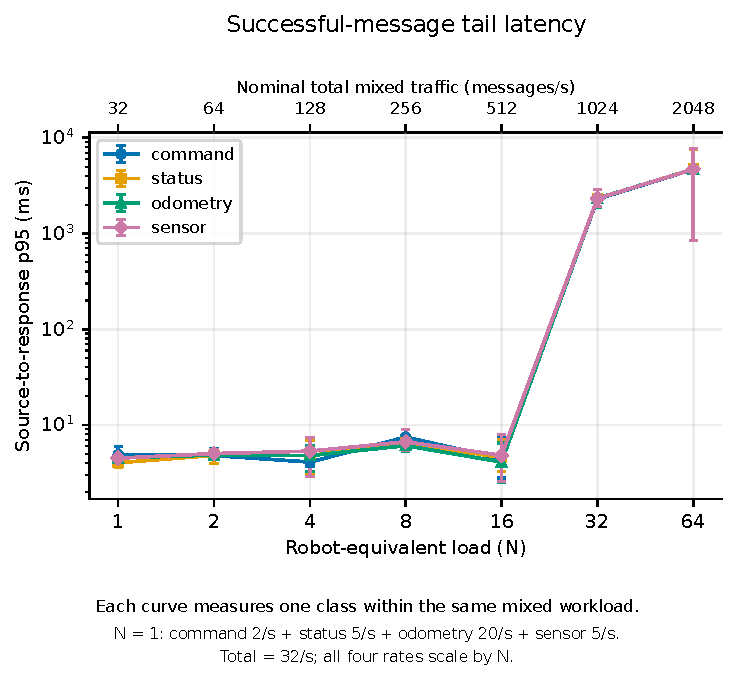
\includegraphics[width=\columnwidth]{fig1_latency.pdf}
    \caption{E1: per-class p95 source-to-response latency versus
    robot-equivalent load $N$.
    The top axis shows nominal total mixed traffic, $32N$ messages/s,
    across all four classes. Each curve reports one class's outcomes under
    that same mixed workload. At $N=1$, command, status, odometry and
    sensor rates are 2, 5, 20 and 5 messages/s; all rates scale by $N$.
    Latency includes successful messages only. Points are means of three
    run-level p95 values; error bars show minimum--maximum. Load and
    latency use logarithmic scales.}
    \label{fig:e1-latency}
\end{figure}

\begin{figure}[tbp]
    \centering
    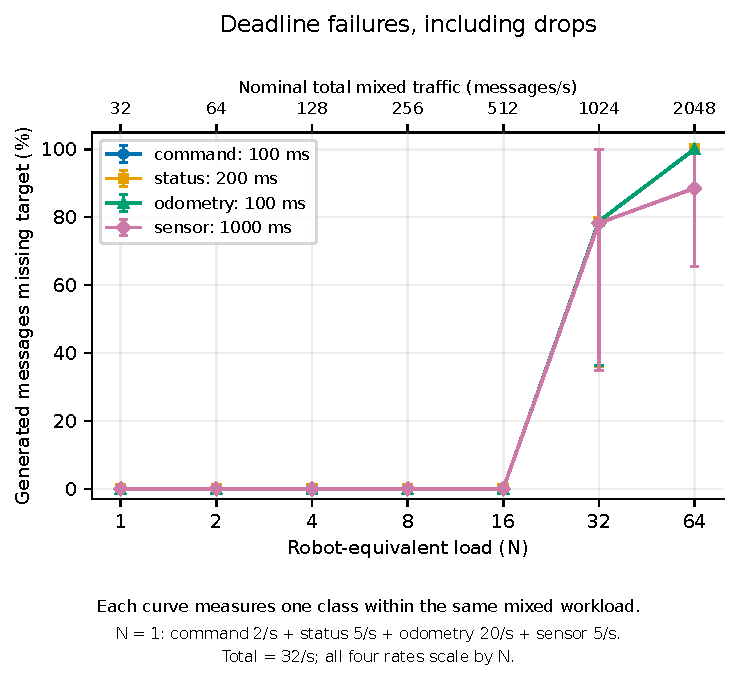
\includegraphics[width=\columnwidth]{fig2_deadlines.pdf}
    \caption{E1: per-class deadline-failure ratio versus robot-equivalent
    load $N$. The top axis shows nominal total mixed traffic, $32N$
    messages/s, across all four classes. At $N=1$, command, status,
    odometry and sensor rates are 2, 5, 20 and 5 messages/s; all rates
    scale by $N$. Each curve reports one class's outcomes under that
    same mixed workload. Failures include late and unsuccessful messages.
    Targets are command 100 ms, status 200 ms, odometry 100 ms and sensor
    1,000 ms. Points are means of three run-level percentages; error bars
    show minimum--maximum. Load uses a logarithmic scale.}
    \label{fig:e1-deadlines}
\end{figure}

\begin{figure}[tbp]
    \centering
    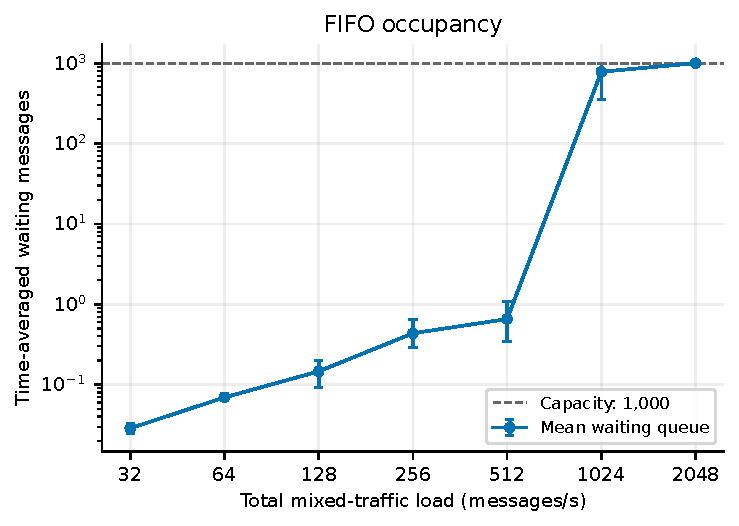
\includegraphics[width=\columnwidth]{fig3_queue.pdf}
    \caption{E1: time-averaged FIFO occupancy versus total mixed-traffic
    load across all four classes. The queue holds 1,000 waiting messages
    and excludes the request in service. Points are means of three runs;
    error bars show minimum--maximum. Offered load and mean queue
    occupancy use logarithmic scales.}
    \label{fig:e1-queue}
\end{figure}

\begin{figure}[tbp]
    \centering
    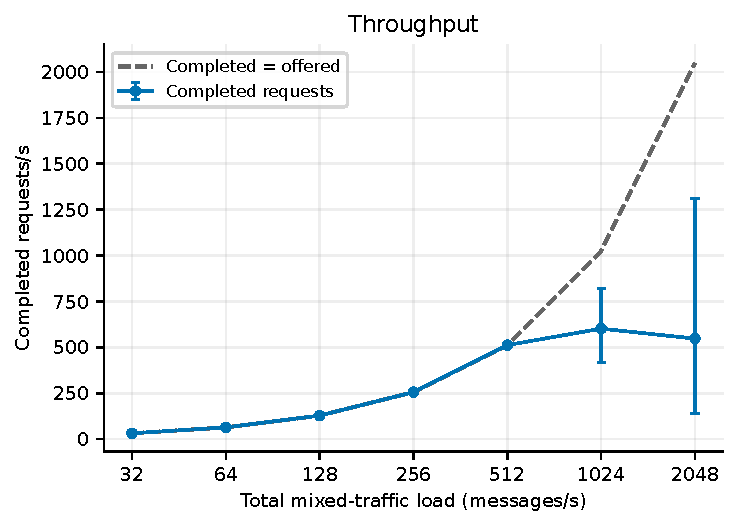
\includegraphics[width=\columnwidth]{fig4_throughput.pdf}
    \caption{E1: completed request throughput versus total mixed-traffic
    load across all four classes. The reference line denotes completion
    rate equal to offered rate. Points are means of three runs; error
    bars show minimum--maximum. Offered load uses a logarithmic scale.}
    \label{fig:e1-throughput}
\end{figure}

\subsubsection{Resource Use and Deadline Performance}
At the highest load, sender occupied time averaged 99.5\%, compared with
39.3\% for the server POST handler (Figure~\ref{fig:e1-busy-time}).
Gateway and server CPU consumption
averaged 114.2\% and 14.7\% of one logical CPU, respectively
(Figure~\ref{fig:e1-cpu}). Averaging the per-run mean delays gave
4,175.88 ms of queue waiting and 3.98 ms for the HTTP exchange. Together,
these measurements implicate the serial gateway/client service path;
they do not show that the server or a physical link reached its capacity.

At this load, mean run-level command p95 latency reached 4,676.28 ms,
and all generated commands failed their 100 ms target
(Figure~\ref{fig:e1-deadlines}). The FIFO baseline
therefore did not protect command deadlines under this stress condition.
Comparisons between classes must account for their different deadline
targets and traffic rates.

\begin{figure}[tbp]
    \centering
    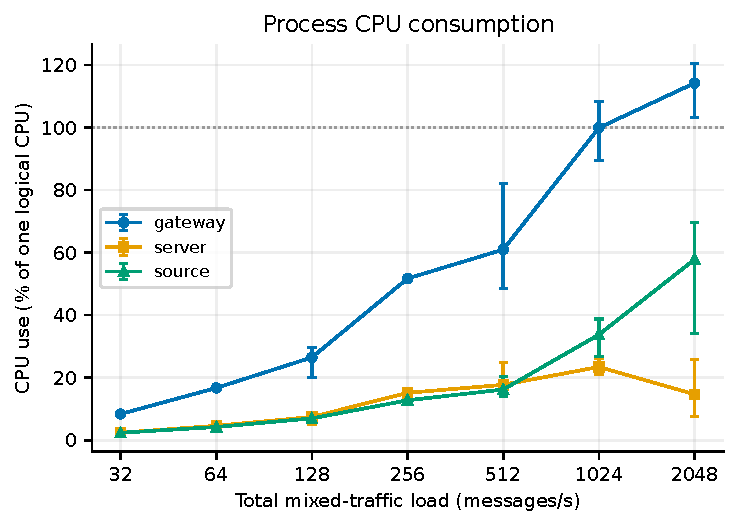
\includegraphics[width=\columnwidth]{fig5_cpu.pdf}
    \caption{E1: process CPU consumption versus total mixed-traffic load
    across all four classes. CPU consumption is normalised to one logical
    CPU and may exceed 100\%. Points are means of three runs; error bars
    show minimum--maximum. CPU consumption is distinct from the occupied
    time shown in Figure~\ref{fig:e1-busy-time}.}
    \label{fig:e1-cpu}
\end{figure}

\begin{figure}[tbp]
    \centering
    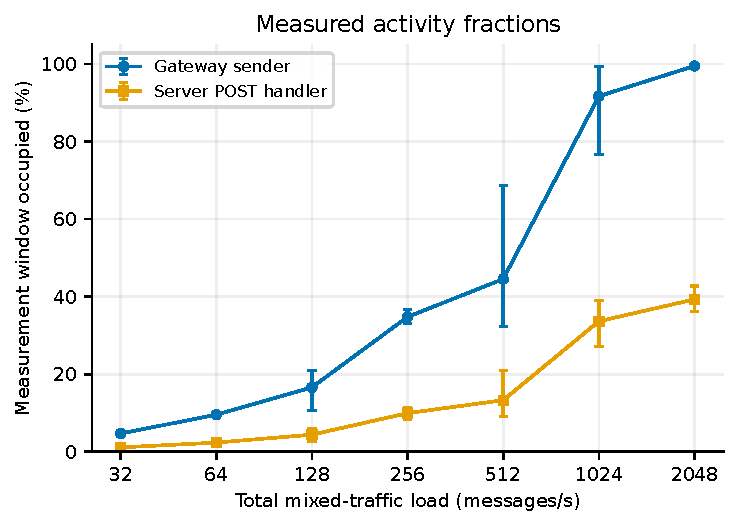
\includegraphics[width=\columnwidth]{fig6_busy_time.pdf}
    \caption{E1: sender and server-handler occupied fractions versus total
    mixed-traffic load across all four classes. Sender activity covers
    dequeue to response completion; server activity covers POST-handler
    entry to response write completion. Points are means of three runs;
    error bars show minimum--maximum. Occupied time is a wall-time measure,
    distinct from CPU consumption.}
    \label{fig:e1-busy-time}
\end{figure}

\subsubsection{Repeat Variability and Reusable Conditions}
At 64 equivalents, completed throughput ranged from 139.1 to 1,309.0
requests/s across repetitions, while run-level p95 latency ranged from
851.40 to 7,649.29 ms. CPU time per message increased across multiple
processes later in the sweep, with a marked change during the first
32-equivalent repetition (Appendix~\ref{app:variability}). The measurements
show variation in shared-host execution performance but do not establish
its cause. All repetitions remain in the reported dataset.

The 16-equivalent condition is the highest tested load with no FIFO drops
in all repetitions, and 64 equivalents provides a repeatable occurrence
of overflow. These are useful reference and stress configurations, but
the results do not establish a single stable service-capacity threshold.
Later comparisons should recheck the reference condition and control or
record host execution variability.

% Uncomment each results subsection only when it has measured evidence.
% For each: state the question, what changed from the shared setup,
% the results with uncertainty, and the interpretation/limitations.
%
% \subsection{E4: Queueing Measurements and Little's Law}
% Match queue/system boundaries and flow populations in L = lambda W.
% With drops, offered rate differs from admitted rate. Address transient
% behaviour, censoring and the periodic/heterogeneous workload assumptions.
%
% \subsection{E2: HTTP/1.1 versus HTTP/2}
% Control workload and document connection count, concurrency, TLS,
% implementation and scheduling so protocol and architecture effects
% can be distinguished. Include command tails and packet evidence.
%
% \subsection{E3: FIFO versus Priority Scheduling}
% Fix protocol and stress load. Include effects on all four classes.
%
% \subsection{E5: Application-Layer Reliable Communication}
% Compare no ARQ, Stop-and-Wait and Selective Repeat. Define injected
% application faults and distinguish them from TCP packet recovery.
%
% \subsection{E6: HTTP/2 versus HTTP/3 under Impairment}
% Workbook matrix: loss 0/1/5 percent crossed with two RTT conditions.
% Report implementation/setup costs as well as steady-state metrics.
%
% \subsection{E7: Scaling to One, Two and Three Server Workers}
% Document actual workers, hosts, balancing and gateway concurrency.
% The E1 sender has one outstanding request and cannot exercise parallel
% service effectively. Discuss M/M/m assumptions rather than assert a fit.
%
% \subsection{E8: Adaptive Gateway Evaluation}
% Compare FIFO, priority and adaptive policies using frozen, unseen
% evaluation conditions. Include command deadlines and sensor freshness.

%==========================================================
\section{Discussion and Limitations}
\label{sec:discussion}

\subsection{What the Baseline Establishes}
The completed experiment demonstrates how this bounded FIFO implementation
behaves under increasing load, including the relationship between waiting,
overflow and missed deadlines. It motivates testing scheduling and client
concurrency in later comparisons. Adding server workers alone cannot be
assumed to improve a path restricted to one outstanding request.

\draftnote{After the remaining experiments, replace this subsection with
a synthesis across them: which changes helped which traffic classes,
under what conditions, and at what cost. Avoid repeating every result.}

\subsection{Threats to Validity}
The shared-host loopback setup does not measure a physical distributed
robot deployment. Rate-scaled robot-equivalents do not reproduce every
effect of adding independent ROS2 nodes or HTTP clients. Periodic traffic
and heterogeneous payloads do not establish the assumptions of an M/M/1
model. Large repeat variability limits capacity claims; three repetitions
and sparse low-load command samples also limit tail-latency precision.
Successful-only latency must be read alongside drops and loss-inclusive
deadline failures. The earlier single-topic pilot dataset is retained as
preliminary evidence and is not pooled with the completed E1 sweep.

%==========================================================
\section{Conclusion}
\label{sec:conclusion}

The implemented baseline completed a seven-load, three-repetition study
of a persistent HTTP/1.1 ROS2-to-REST gateway. The 16-equivalent condition
had no FIFO drops in any repetition, whereas every 32- and 64-equivalent
run overflowed the queue. At the highest load, queue waiting dominated
latency and all command messages failed their deadline target. These
findings establish reference and stress conditions for later experiments,
subject to the substantial variation observed in shared-host performance.

\draftnote{Rewrite the conclusion and abstract together after the full
project is complete. Answer the research questions using only measured
comparisons; distinguish unfinished planned work from demonstrated results.}

\printbibliography

%==========================================================
\clearpage
\onecolumn
\appendix

\section{Additional E1 Evidence}
\label{app:variability}

Figures~\ref{fig:within-run-cpu} and~\ref{fig:within-run-queue} show changes
in process CPU consumption and queue occupancy during the first
32-equivalent repetition. This evidence supports
reporting the observed execution variability without assigning an
unmeasured cause. The accompanying dataset retains all 21 run-level
results in \inlinecode{individual\_runs.csv}.

\begin{figure}[tbp]
    \centering
    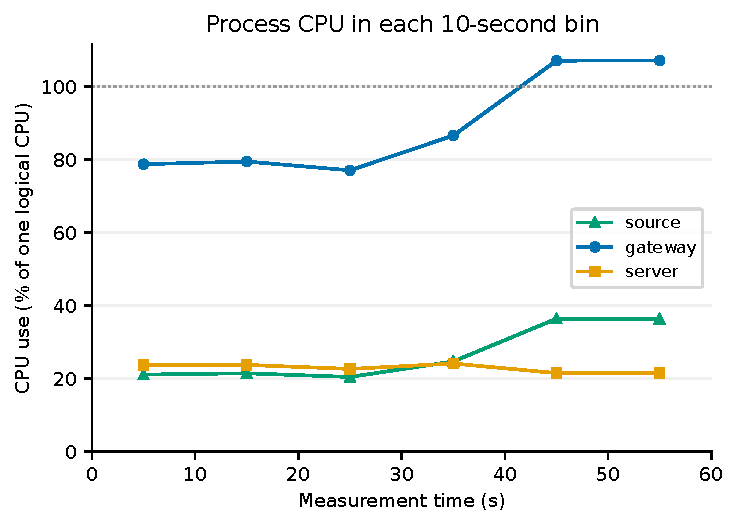
\includegraphics[width=\columnwidth]{appendix_within_run_cpu.pdf}
    \caption{Process CPU consumption in consecutive 10-second intervals
    of the first 32-equivalent repetition. The within-run change
    is retained as evidence of variability; no causal attribution is made.}
    \label{fig:within-run-cpu}
\end{figure}

\begin{figure}[tbp]
    \centering
    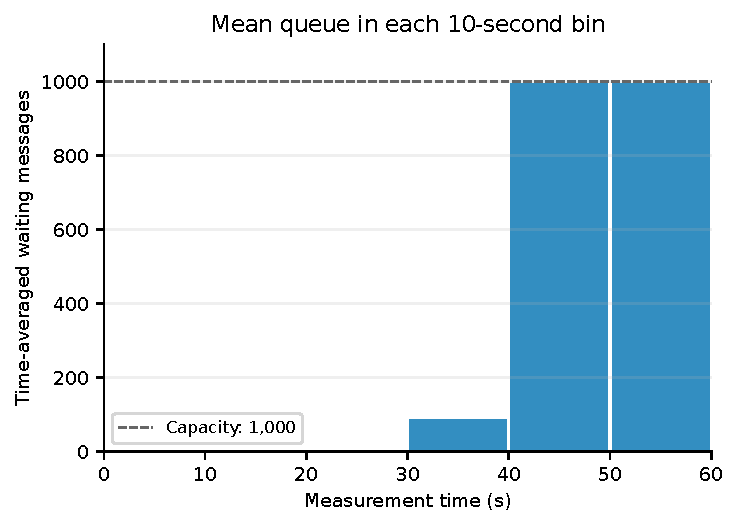
\includegraphics[width=\columnwidth]{appendix_within_run_queue.pdf}
    \caption{Mean FIFO occupancy in consecutive 10-second intervals of the
    first 32-equivalent repetition. Queue growth coincides with the CPU
    changes shown in Figure~\ref{fig:within-run-cpu}; this does not establish
    their cause. The queue holds 1,000 waiting messages.}
    \label{fig:within-run-queue}
\end{figure}

\section{Configurations, API and Reproduction}
\label{app:reproduce}

\draftnote{Add the API/message schema, exact commands, environment versions,
configuration and source hashes, dataset location and selected packet
evidence. Keep long configuration listings here rather than in the main
results. Reference the capture's measurement scope and avoid interpreting
loopback accounting as physical Ethernet wire overhead.}

% Useful project sources for this appendix:
% experiments/E1_PROTOCOL.md
% experiments/baseline.json
% experiments/e1_reference.json
% experiments/e1_stress.json
% results/e1_complete/individual_runs.csv
% results/e1_complete/variability_note.md
% results/e1_packet_evidence/README.md
% README.md (build/run/analyse instructions)

\end{document}
